\documentclass[12pt]{article}
\usepackage[margin=1in]{geometry}                % See geometry.pdf to learn the layout options. There are lots.
\geometry{letterpaper}                   % ... or a4paper or a5paper or ... 
\usepackage{graphicx}
\usepackage[usenames,dvipsnames]{color}
\usepackage{amssymb}
\usepackage{epstopdf}
\usepackage{verbatim}
\usepackage{listings}
\lstset{language=Java,
	basicstyle=\ttfamily,
	keywordstyle=\color{blue}\ttfamily,
	stringstyle=\color{red}\ttfamily,
	showstringspaces=false,
	commentstyle=\color{ForestGreen}\ttfamily,
	morecomment=[l][\color{magenta}]{\#}}
\DeclareGraphicsRule{.tif}{png}{.png}{`convert #1 `dirname #1`/`basename #1 .tif`.png}
\usepackage{fancyhdr}
\pagestyle{fancy}
\fancyhf{}
\fancyhead[R]{\thepage}

\title{CSE 430 Summer 2014 - Project 3}
\author{Ryan Dougherty - ASU ID: 1203621947}
\date{}                                           % Activate to display a given date or no date

\newcommand{\imagesize}{100mm}

\begin{document}
\maketitle

\tableofcontents

\abstract{This document will cover Project 3, which is about making use of the Ubuntu distribution of Linux. We will use VMWare, a virtual machine, that allows Ubuntu to be installed on the host OS. We will install build the latest kernel, and then run some applications on Ubuntu. This report will detail the findings during installation and running.}

\section{Installing Ubuntu}
After installing VMWare Fusion (trial version), we have to install the virtual machine for the Ubuntu Operating System:

\begin{figure}[ht!]
\centering
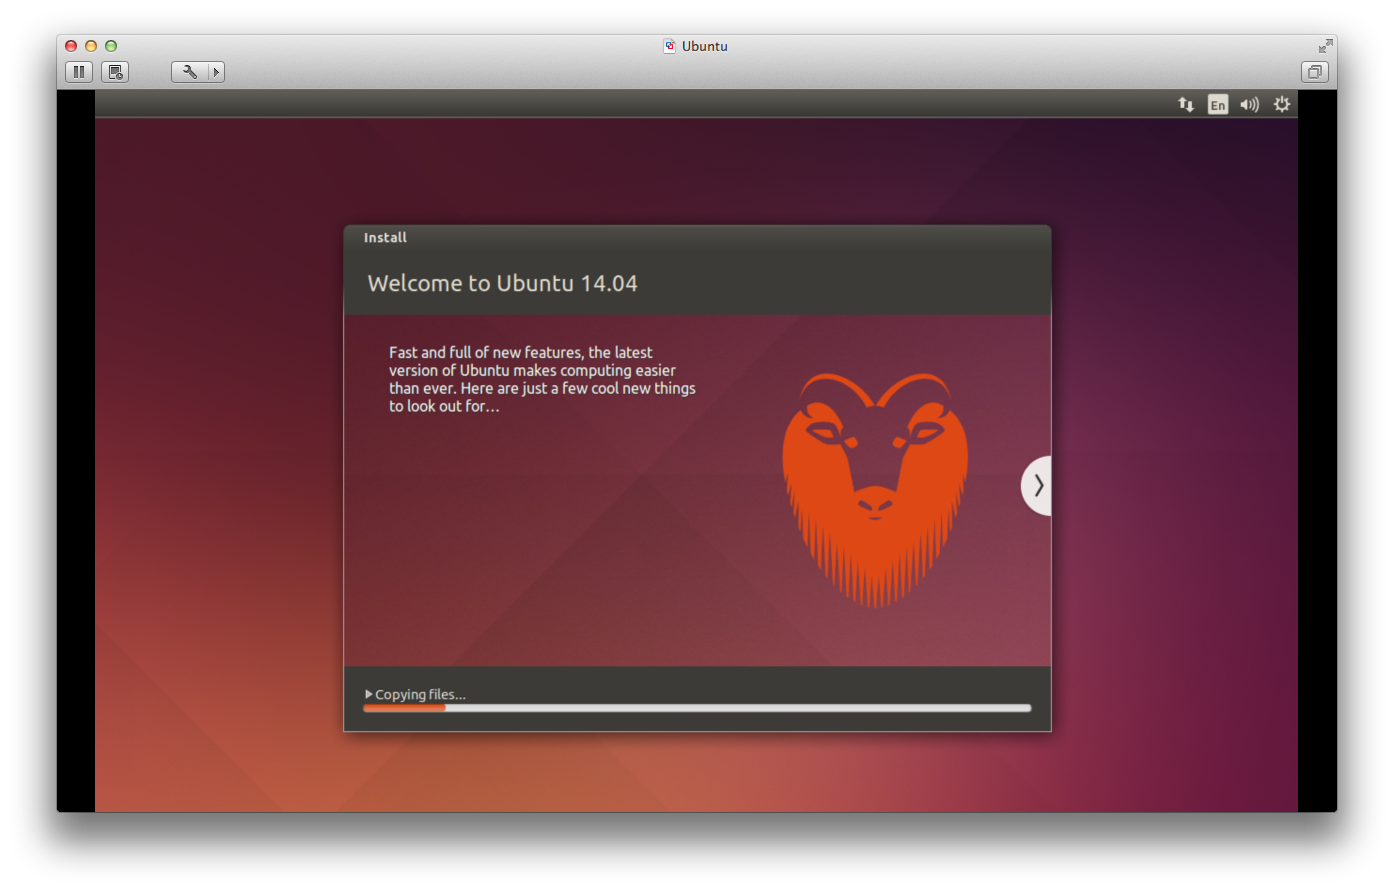
\includegraphics[width=\imagesize]{1.jpg}
\caption{Installing Ubuntu}
\end{figure}

\begin{figure}[ht!]
\centering
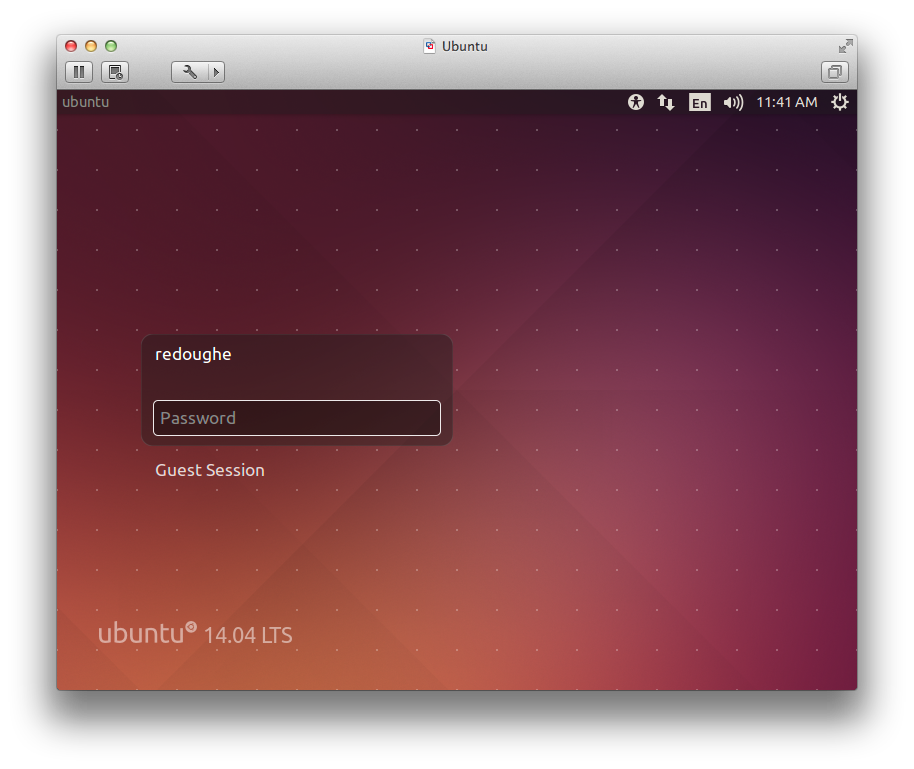
\includegraphics[width=\imagesize]{2.jpg}
\caption{Ubuntu Login Screen}
\end{figure}

\newpage

We then run Software Updater to make sure that everything is up-to-date. The purpose of this is to have the OS be current and avoid possible problems in the installation process.

\begin{figure}
\centering
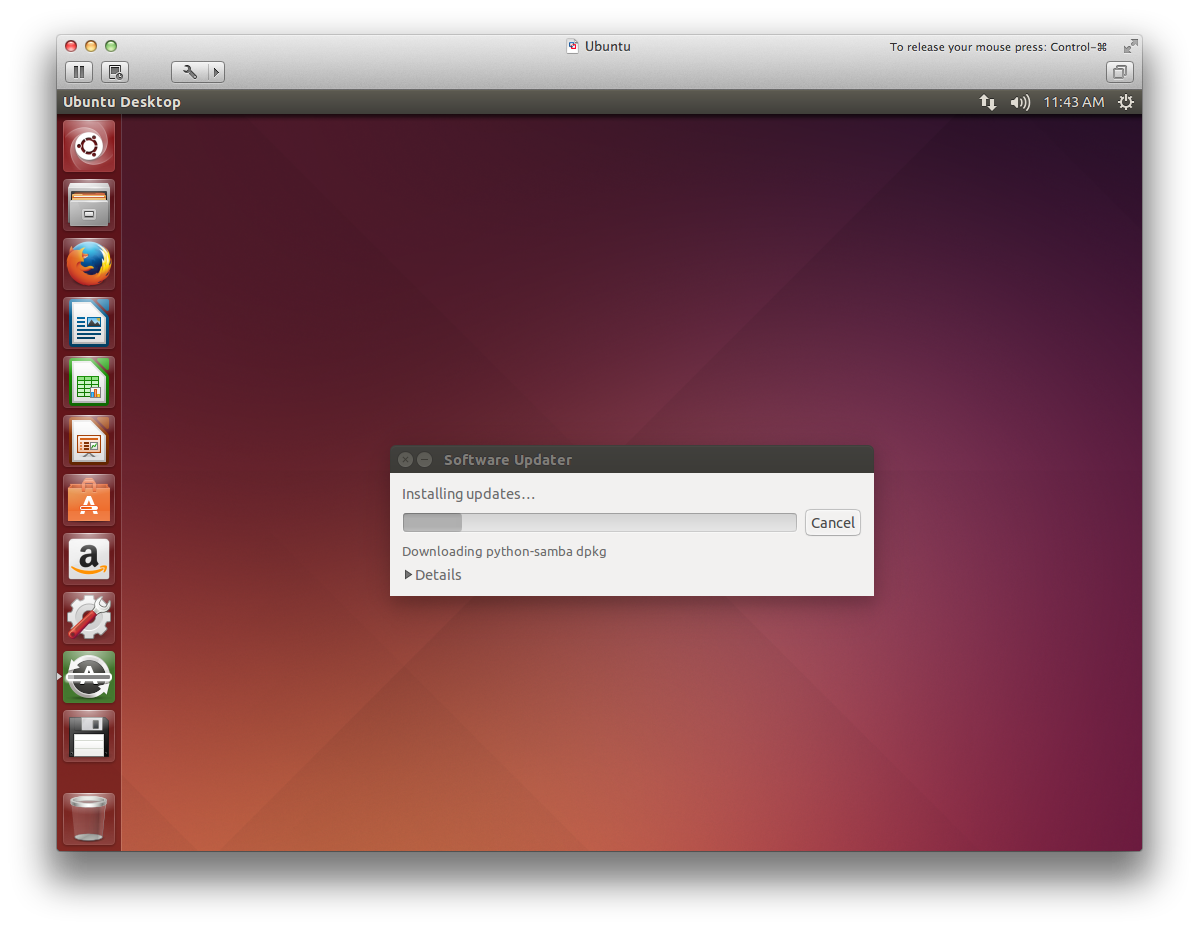
\includegraphics[width=\imagesize]{3.jpg}
\caption{Running Software Updater}
\end{figure}

\newpage 

\section{Kernel Development Directory}

After installing Ubuntu, what we need to do is to create a directory for kernel development, by executing the commands:
\begin{verbatim}
mkdir cse430
cd cse430
\end{verbatim}

\begin{figure}
\centering
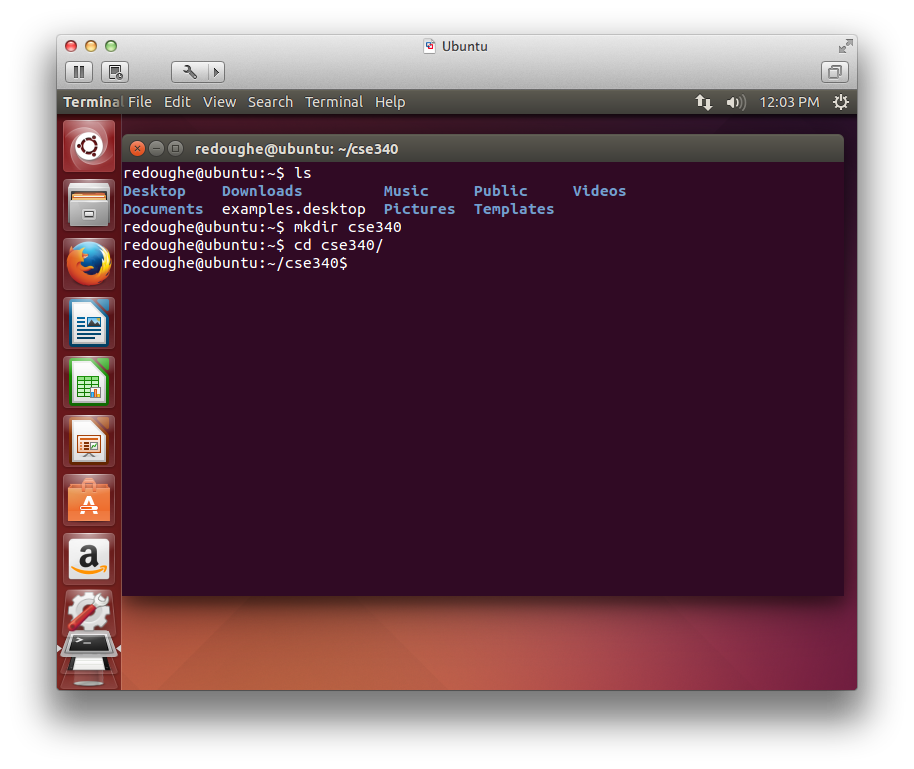
\includegraphics[width=\imagesize]{4.jpg}
\caption{Making the directory}
\end{figure}

\newpage

\section{Utilities for Packaging Kernel}
We now download and install the utilities needed to perform the compilation and packaging of the kernel, by executing the following commands:

\begin{verbatim}
sudo apt-get update
sudo apt-get install dpkg-dev kernel-package gcc libc6-dev 
        binutils make bin86 module-init-tools gawk gzip grep libncurses5-dev
\end{verbatim}

\begin{figure}
\centering
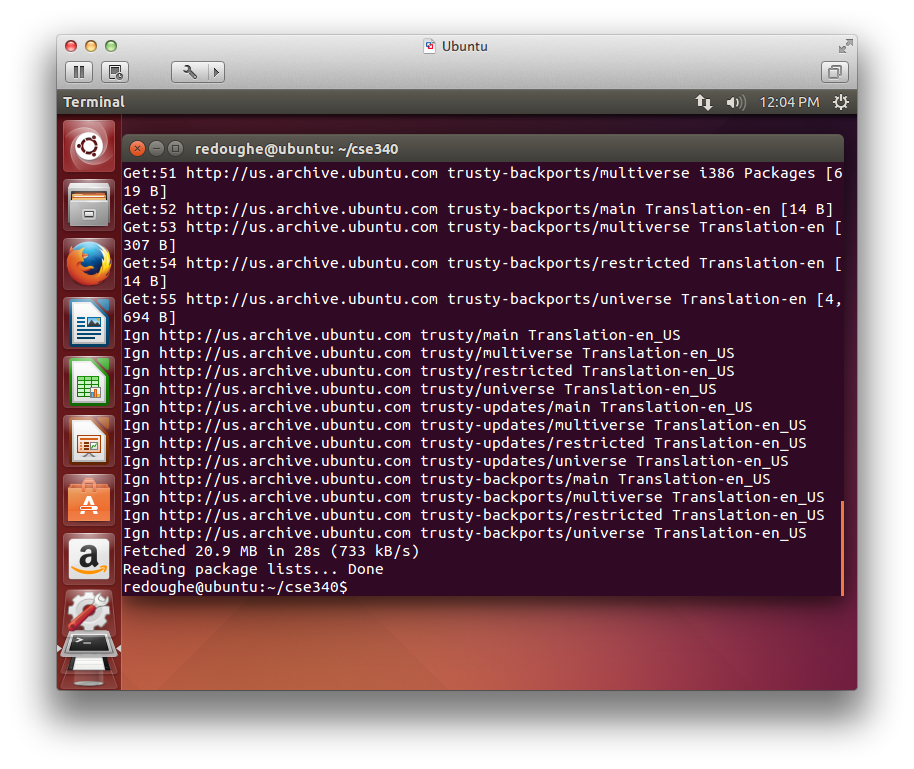
\includegraphics[width=\imagesize]{5.jpg}
\caption{Executing the apt-get commands above}
\end{figure}

\newpage

\section{Decompressing Kernel Source Code}
We now download and decompress the source code for the latest Ubuntu kernel from the source tree, by executing the following command:

\begin{verbatim}
apt-get source linux-image-$(uname -r)
\end{verbatim}

\begin{figure}
\centering
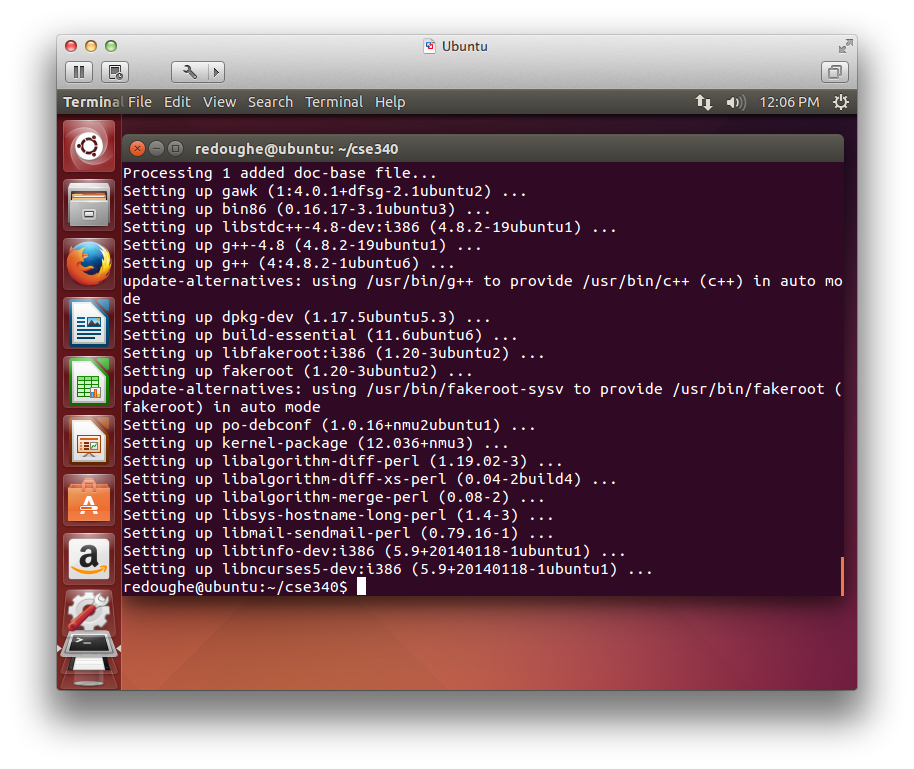
\includegraphics[width=\imagesize]{6.jpg}
\caption{Downloading and decompressing Ubuntu kernel}
\end{figure}

\newpage

\section{Configuring the Kernel}
Now is the step to configure the kernel. We change the working directory to the top level of the source directory for the kernel. Then we configure the kernel. Then we clean the build environment. The following commands are to be executed:

\begin{verbatim}
cd linux-3.5.0 (or whatever version is loaded)
make menuconfig
make-kpkg clean
fakeroot make-kpkg --initrd --revision=1.0.cse430 kernel_image
\end{verbatim}

The last command took over 2 hours to execute, which is more than I expected. It made me realize how complicated kernel code and software packages can really be, since most packages I have installed before took almost no considerable time.

\begin{figure}
\centering
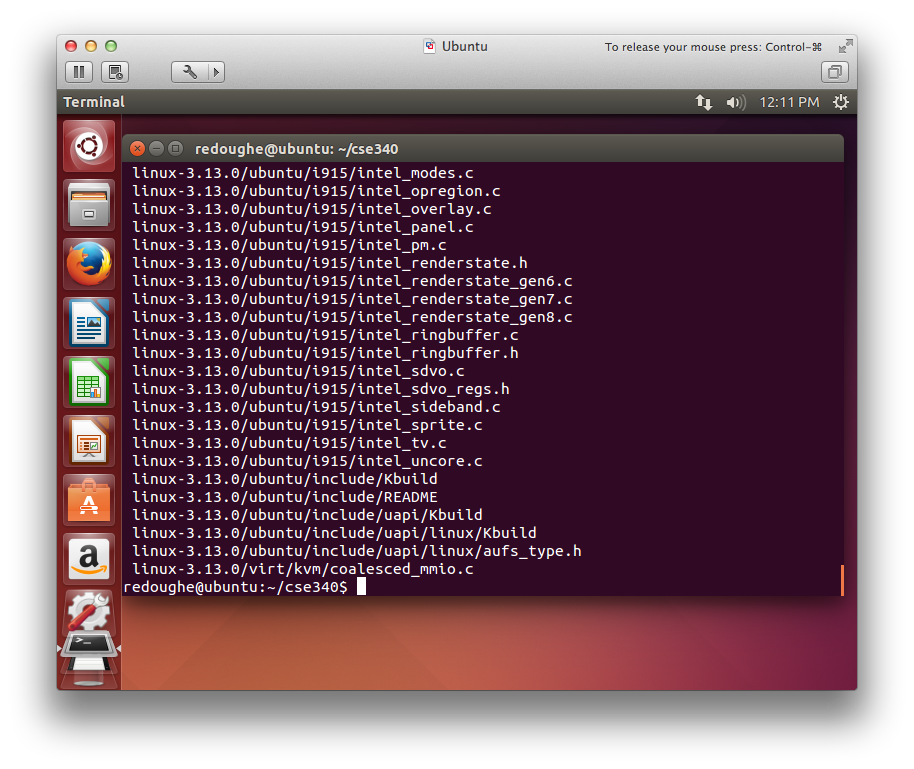
\includegraphics[width=\imagesize]{7.jpg}
\caption{Executing first three commands}
\end{figure}

\begin{figure}
\centering
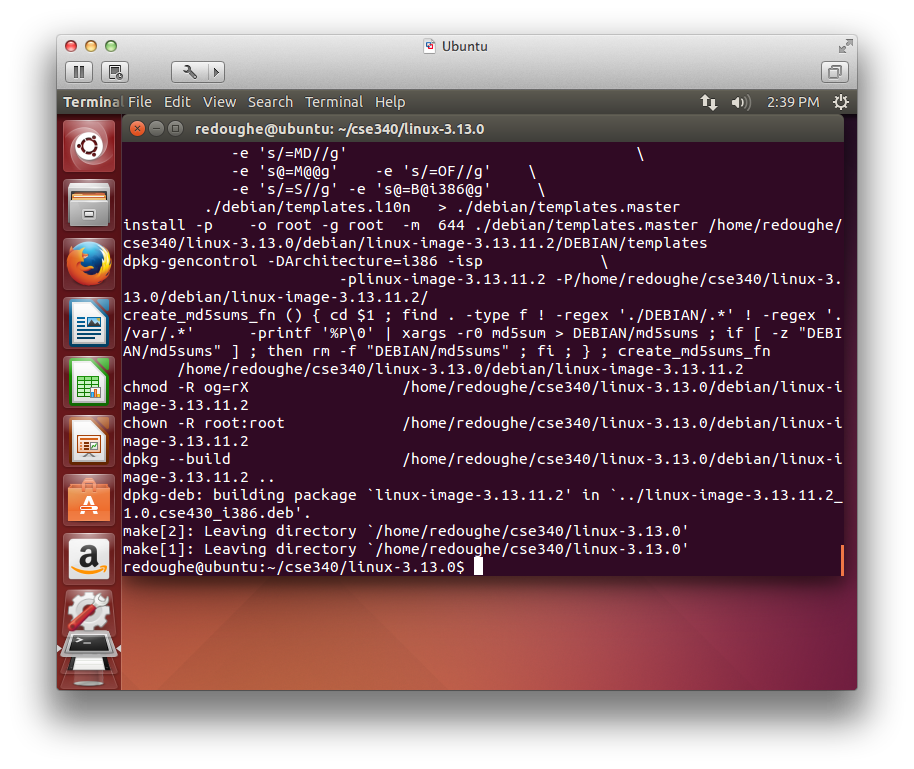
\includegraphics[width=\imagesize]{8.jpg}
\caption{Executing last command}
\end{figure}

\newpage

\section{Current OS Revision / Updating Kernel}
We now show the current version of our OS, and then update the kernel (and reboot). The commands are:

\begin{verbatim}
cat /proc/version
sudo dpkg -i ../linux-image-3.5.7.2_1.0.cse430_i386.deb
sudo shutdown -r now
cat /proc/version
\end{verbatim}

\begin{figure}
\centering
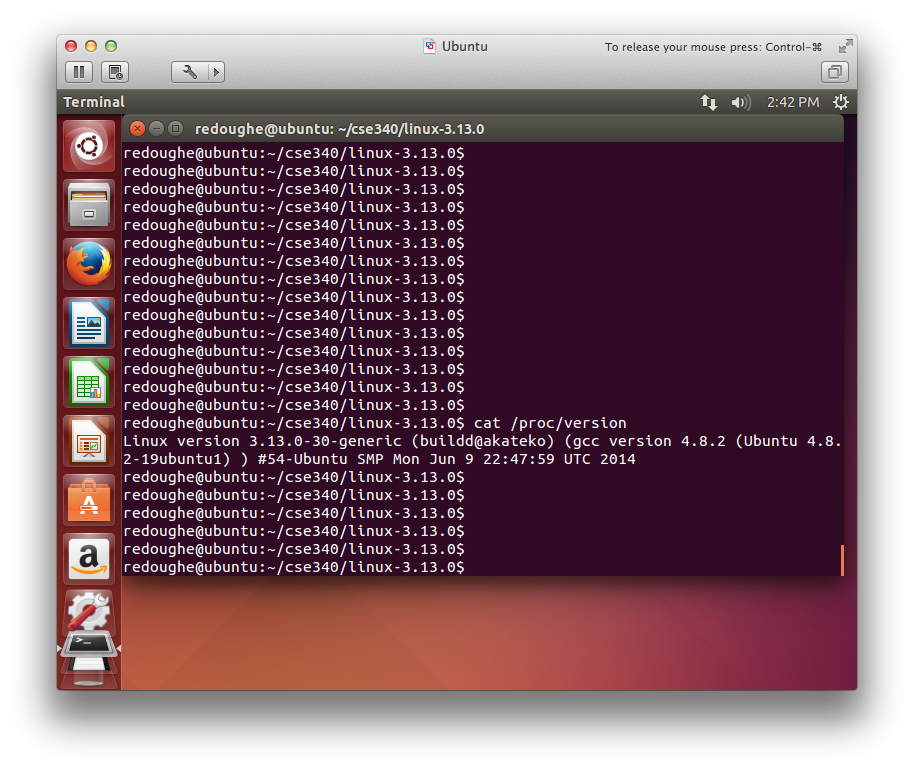
\includegraphics[width=\imagesize]{9.jpg}
\caption{Showing current OS version}
\end{figure}

\begin{figure}
\centering
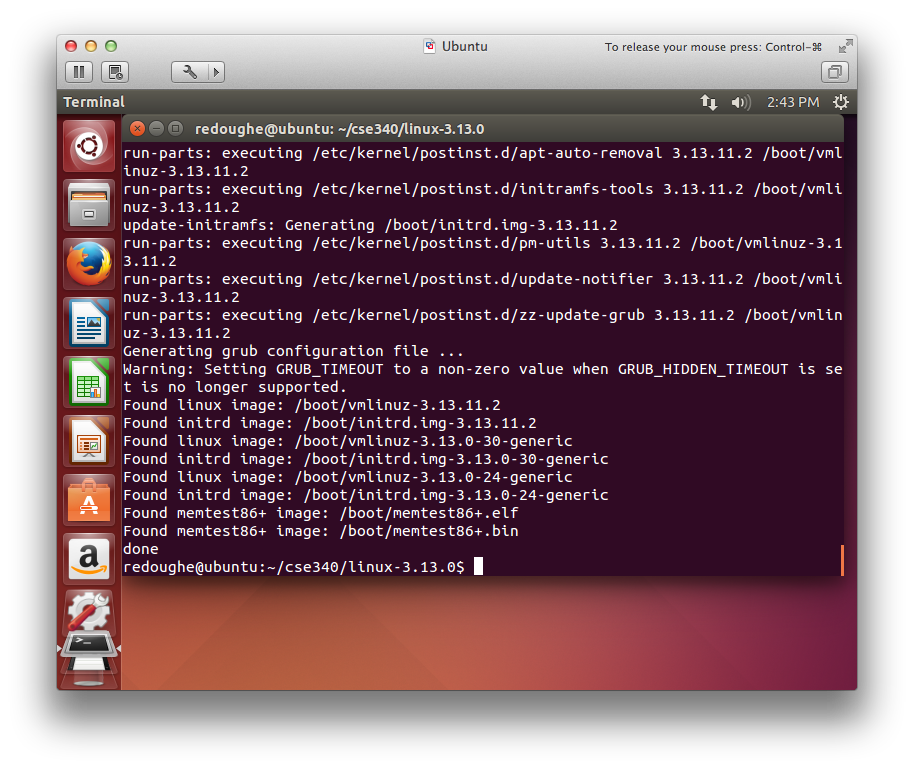
\includegraphics[width=\imagesize]{10.jpg}
\caption{Running 2nd command}
\end{figure}

\begin{figure}
\centering
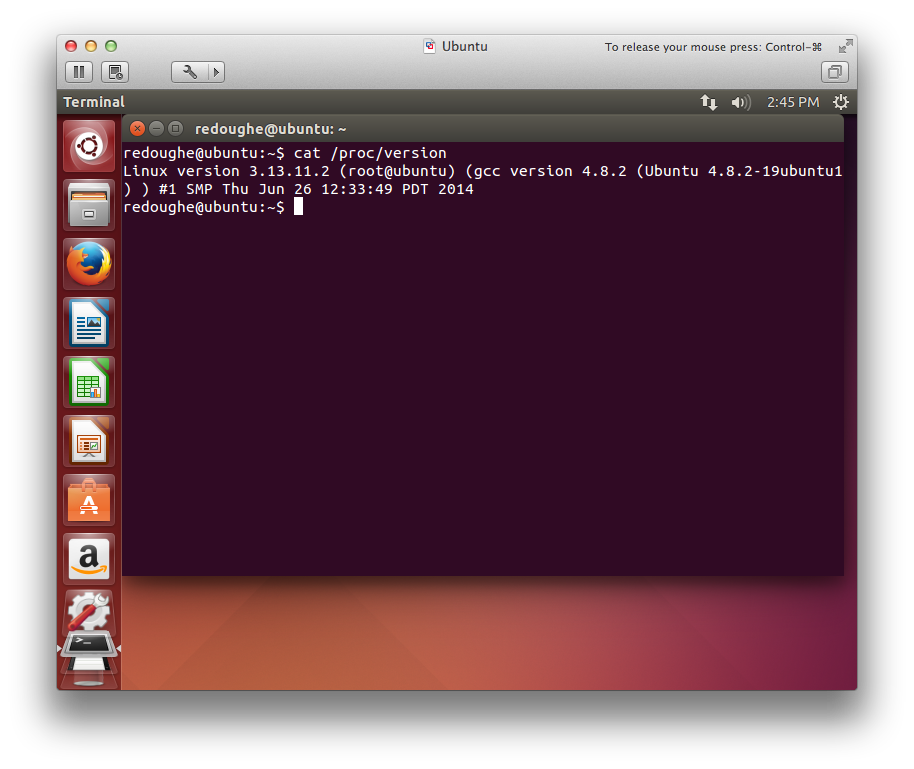
\includegraphics[width=\imagesize]{11.jpg}
\caption{Showing current OS version after reboot}
\end{figure}

\newpage

\section{Running applications}
Finally, we show running various applications withing Ubuntu. The applications that were used were Chromium, a web browser; Calculator; and LibreOffice.

\begin{figure}
\centering
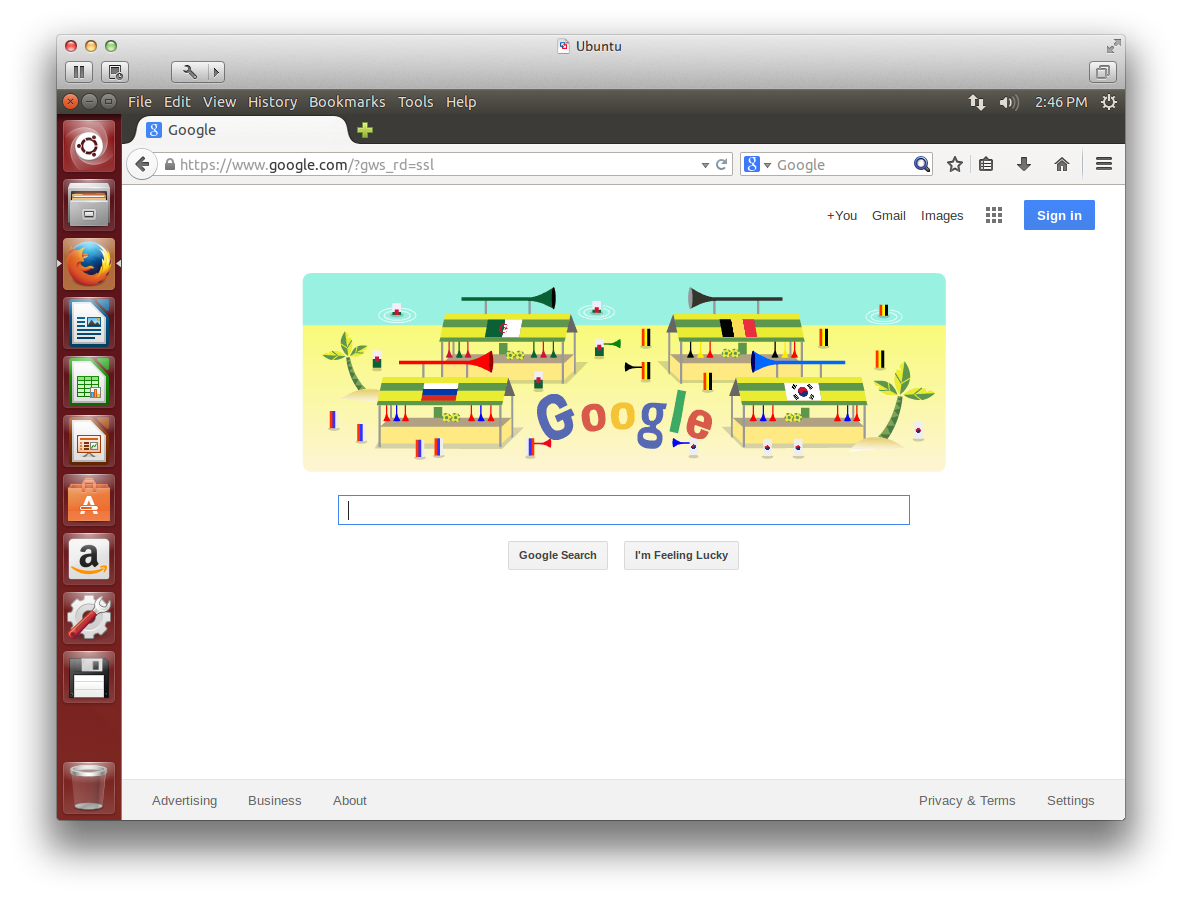
\includegraphics[width=\imagesize]{12.jpg}
\caption{Running Chromium}
\end{figure}

\begin{figure}
\centering
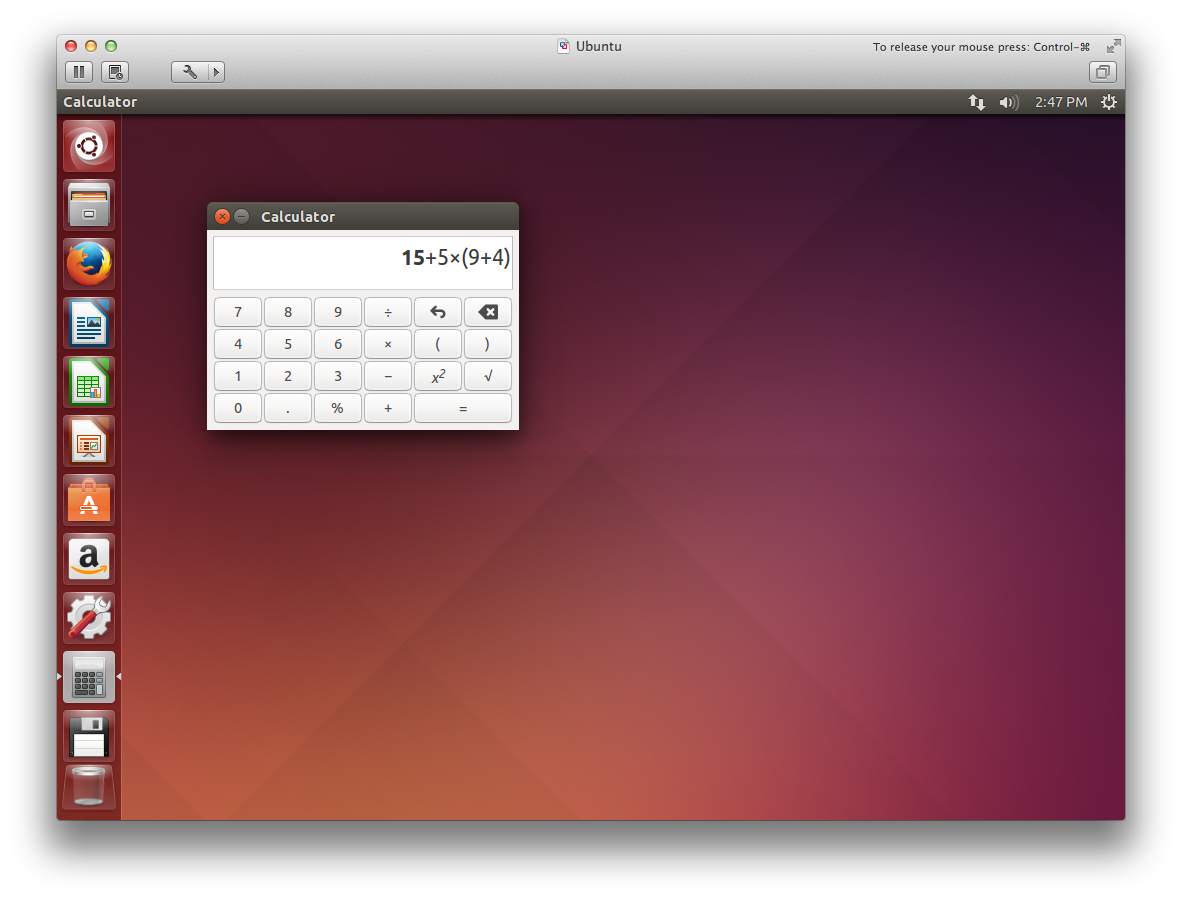
\includegraphics[width=\imagesize]{13.jpg}
\caption{Running Calculator}
\end{figure}

\begin{figure}
\centering
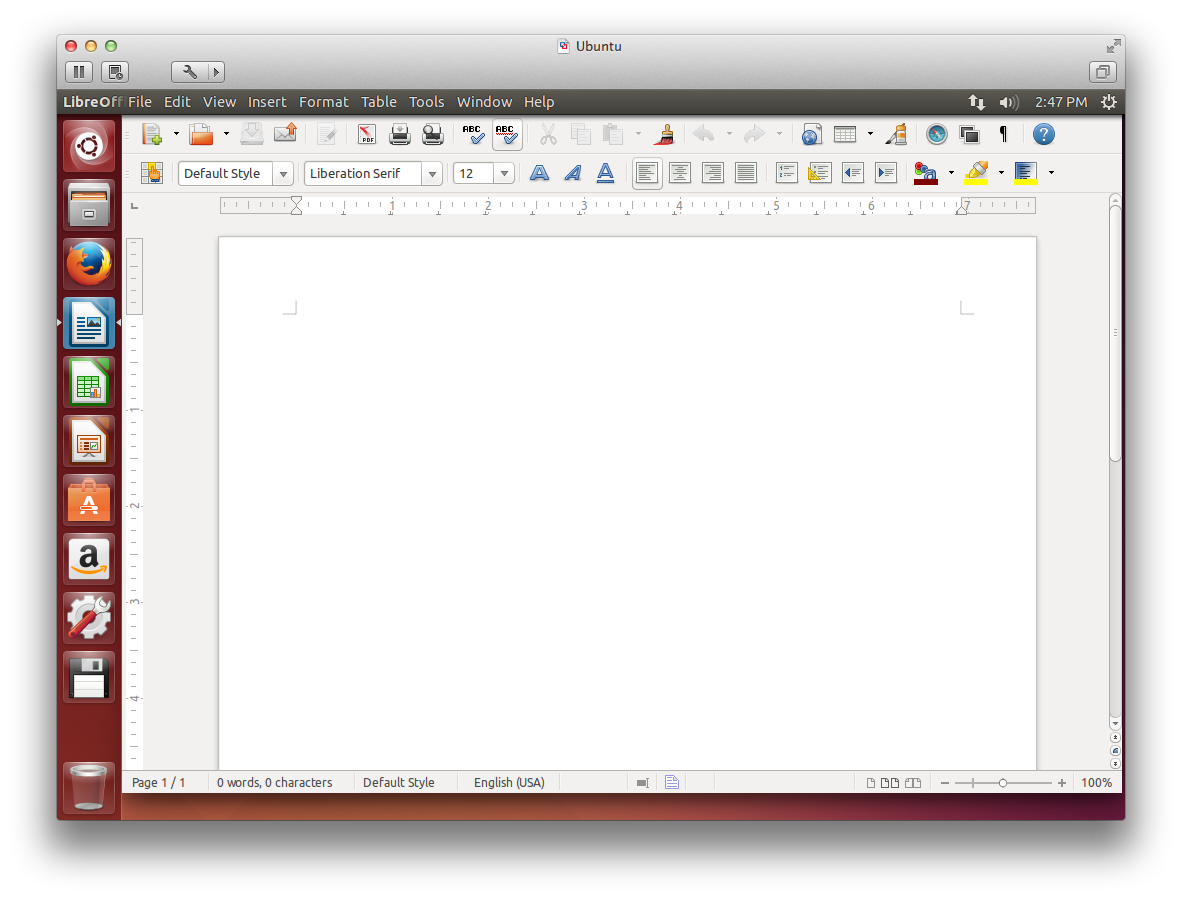
\includegraphics[width=\imagesize]{14.jpg}
\caption{Running LibreOffice}
\end{figure}

\newpage

\section{Conclusions}
Ubuntu (or more generally, Linux) is an operating system that I have not used before. I currently use Mac OS X and sometimes use Windows. A lot of the commands and setup were very easy to use, and I like many of the built-in applications that came with Ubuntu. In Mac OS X, I use Terminal, which is basically the same program/interface provided in Ubuntu.
\\ \\
Many of the advantages of Ubuntu, such as its being free, widely used, very fast, and many others make me reconsider my primary operating system choice. 

\end{document}  